% !TEX root = ../Main.tex
\chapter{垂直关系}

与"平行"对称，"垂直"也是\textbf{三层}体系：线线垂直、线面垂直、面面垂直。核心思想仍然是——\textbf{利用判定与性质定理在三层之间来回跳转}。不过垂直判定比平行\textbf{更"强力"}：线面垂直之后可以反推到所有方向的线线垂直。

\section{线线垂直}

\state{异面直线的垂直}{
    空间中两直线 $a, b$（相交或异面）\textbf{垂直}，指的是把它们\textbf{平移到同一点相交}后所成的角为 $90^\circ$。即：$a \perp b$ 等价于两直线的\textbf{方向向量}互相垂直。
}

\state{线线垂直的常见来源}{
    \begin{enumerate}
        \item[\textbf{(i)}] \textbf{线面垂直反推}：若 $\ell \perp \alpha$，则 $\ell$ 垂直于 $\alpha$ 内\textbf{所有}直线——这是最强的垂直来源；
        \item[\textbf{(ii)}] \textbf{等腰/菱形的对角线}：底边中线 $\perp$ 底边、菱形对角线互相垂直；
        \item[\textbf{(iii)}] \textbf{直径的圆周角}：直径所对的圆周角是直角（证直角三角形）；
        \item[\textbf{(iv)}] \textbf{向量法}：证 $\vec{AB} \cdot \vec{CD} = 0$。
    \end{enumerate}
}

\section{线面垂直}

\state{线面垂直判定定理}{
    \textbf{判定}：若 $\ell$ 与平面 $\alpha$ 内\textbf{两条相交直线} $a, b$ 都垂直，则 $\ell \perp \alpha$。

    用文字：\textbf{一条直线与一个平面内的两条相交直线都垂直，则此直线与此平面垂直。}

    \textbf{注意}：\textbf{相交}是本质要求——若只与两条平行线垂直，不足以推出线面垂直。
}

\begin{center}
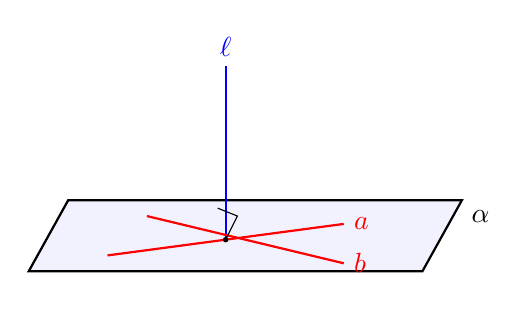
\begin{tikzpicture}[scale=1]
    \draw[thick, fill=blue!5] (-2.5, -0.4) -- (2.5, -0.4) -- (3, 0.5) -- (-2, 0.5) -- cycle;
    \coordinate (O) at (0, 0);
    \draw[thick, blue] (O) -- (0, 2.2) node[above] {$\ell$};
    \draw[thick, red] (-1.5, -0.2) -- (1.5, 0.2) node[right] {$a$};
    \draw[thick, red] (-1, 0.3) -- (1.5, -0.3) node[right] {$b$};
    \draw[thin] (0, 0) -- (0.15, 0.3) -- (-0.1, 0.4);
    \node at (3, 0.3) [right] {$\alpha$};
    \fill (O) circle (1pt);
\end{tikzpicture}
\end{center}

\state{线面垂直的性质}{
    \begin{enumerate}
        \item[\textbf{(i)}] \textbf{垂直即与面内所有线垂直}：$\ell \perp \alpha \implies \ell \perp a$ 对每条 $a \subset \alpha$ 成立；
        \item[\textbf{(ii)}] \textbf{垂直于同一平面的两线平行}：$a \perp \alpha, b \perp \alpha \implies a \parallel b$；
        \item[\textbf{(iii)}] \textbf{垂直于两平行平面的直线同向}：若 $\alpha \parallel \beta$，则 $\ell \perp \alpha \Leftrightarrow \ell \perp \beta$。
    \end{enumerate}
}

\section{三垂线定理}

\state{三垂线定理}{
    设 $P$ 为平面 $\alpha$ 外一点，$PO \perp \alpha$（$O$ 为垂足），$A$ 为 $\alpha$ 内任意一点，$\ell$ 为 $\alpha$ 内过 $A$ 的一条直线。若 \textbf{$OA \perp \ell$}（在 $\alpha$ 内），则 $PA \perp \ell$。

    \textbf{逆定理}：若 $PA \perp \ell$，则 $OA \perp \ell$。
}

\begin{center}
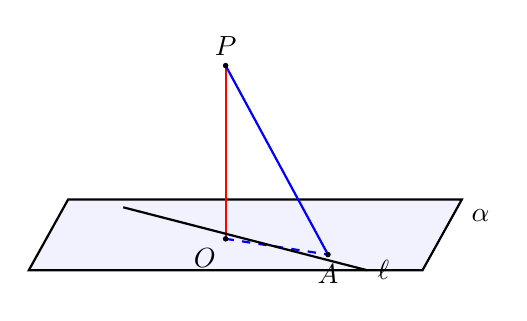
\begin{tikzpicture}[scale=1]
    \draw[thick, fill=blue!5] (-2.5, -0.4) -- (2.5, -0.4) -- (3, 0.5) -- (-2, 0.5) -- cycle;
    \coordinate (O) at (0, 0);
    \coordinate (P) at (0, 2.2);
    \coordinate (A) at (1.3, -0.2);
    \draw[thick, red] (P) -- (O);
    \draw[thick, blue] (P) -- (A);
    \draw[thick, blue, dashed] (O) -- (A);
    \draw[thick] (-1.3, 0.4) -- (1.8, -0.4) node[right] {$\ell$};
    \fill (O) circle (1pt) node[below left] {$O$};
    \fill (P) circle (1pt) node[above] {$P$};
    \fill (A) circle (1pt) node[below] {$A$};
    \node at (3, 0.3) [right] {$\alpha$};
\end{tikzpicture}
\end{center}

\rmkb{
    \textbf{三垂线定理的用途}：把平面内看不清的\textbf{斜线与直线的垂直}，转化为平面内易看的\textbf{"垂足连线与直线"的垂直}。是"空间垂直 $\leftrightarrow$ 平面垂直"的转化桥梁。
}

\section{面面垂直}

\state{二面角与面面垂直}{
    \textbf{二面角}$\alpha$-$\ell$-$\beta$ 的\textbf{平面角}：在棱 $\ell$ 上任取一点 $O$，在 $\alpha$ 内作 $OA \perp \ell$，在 $\beta$ 内作 $OB \perp \ell$，则 $\angle AOB$ 就是二面角的平面角。

    若 $\angle AOB = 90^\circ$，即\textbf{二面角为直角}，则称两平面\textbf{互相垂直}，记 $\alpha \perp \beta$。
}

\state{面面垂直判定定理}{
    \textbf{判定}：若一个平面\textbf{包含}另一个平面的\textbf{垂线}，即 $\ell \subset \beta$ 且 $\ell \perp \alpha$，则 $\alpha \perp \beta$。

    用文字：\textbf{一个平面过另一个平面的一条垂线，则这两个平面互相垂直。}
}

\state{面面垂直性质定理}{
    \textbf{性质}：若 $\alpha \perp \beta$，$\alpha \cap \beta = \ell$，$a \subset \alpha$ 且 $a \perp \ell$，则 $a \perp \beta$。

    用文字：\textbf{两平面互相垂直，则一个平面内垂直于交线的直线垂直于另一个平面。}

    \textbf{这是面面垂直最重要的"使用方式"}——有面面垂直条件时，可在一个面内作交线的垂线，立即得到一条线面垂直。
}

\rmkb{
    \textbf{垂直判定"金三角"}：
    \begin{center}
    \begin{tikzpicture}[scale=1.0]
        \node (l) at (0, 1.2) {\textbf{线线垂直}};
        \node (p) at (-2, -0.5) {\textbf{线面垂直}};
        \node (pp) at (2, -0.5) {\textbf{面面垂直}};
        \draw[<->, thick] (l) -- (p) node[midway, above left] {\small 两相交线};
        \draw[<->, thick] (l) -- (pp) node[midway, above right] {\small 向量 / 平面角};
        \draw[<->, thick] (p) -- (pp) node[midway, below] {\small 含垂线/作交线垂线};
    \end{tikzpicture}
    \end{center}

    \textbf{做题常用套路}：
    \begin{itemize}
        \item 要证 \textbf{线面垂直}——找面内两条相交线各证一次线线垂直；
        \item 要证 \textbf{面面垂直}——在其中一个面内找一条直线，证其垂直于另一个面；
        \item 要证 \textbf{线线垂直}——若能推出一条直线垂直于包含另一条直线的某个面，立得；
        \item 有 \textbf{面面垂直条件}时——\textbf{立刻}想到"作交线垂线"得线面垂直。
    \end{itemize}
}
